\let\negmedspace\undefined
\let\negthickspace\undefined
\documentclass[journal]{IEEEtran}
\usepackage[a5paper, margin=10mm, onecolumn]{geometry}
\usepackage{lmodern} % Ensure lmodern is loaded for pdflatex
\usepackage{tfrupee} % Include tfrupee package

\setlength{\headheight}{1cm} % Set the height of the header box
\setlength{\headsep}{0mm}     % Set the distance between the header box and the top of the text

\usepackage{gvv-book}
\usepackage{gvv}
\usepackage{cite}
\usepackage{amsmath,amssymb,amsfonts,amsthm}
\usepackage{algorithmic}
\usepackage{graphicx}
\usepackage{textcomp}
\usepackage{xcolor}
\usepackage{txfonts}
\usepackage{listings}
\usepackage{enumitem}
\usepackage{mathtools}
\usepackage{gensymb}
\usepackage{comment}
\usepackage[breaklinks=true]{hyperref}
\usepackage{tkz-euclide} 
\usepackage{listings}                                      
\def\inputGnumericTable{}                                 
\usepackage[latin1]{inputenc}                                
\usepackage{color}                                            
\usepackage{array}                                            
\usepackage{longtable}
\usepackage{multicol}
\usepackage{calc}                                             
\usepackage{multirow}                                         
\usepackage{hhline}                                           
\usepackage{ifthen}                                           
\usepackage{lscape}
\begin{document}

\bibliographystyle{IEEEtran}
\vspace{3cm}

\title{10.3.2.2.3}
\author{EE24BTECH11010 - Balaji B}
% \maketitle
% \newpage
% \bigskip
{\let\newpage\relax\maketitle}

\renewcommand{\thefigure}{\theenumi}
\renewcommand{\thetable}{\theenumi}
\setlength{\intextsep}{10pt} % Space between text and floats


\numberwithin{equation}{enumi}
\numberwithin{figure}{enumi}
\renewcommand{\thetable}{\theenumi}


\textbf{Question}:\newline
Find out whether the lines $6x-3y+10=0$ and $2x-y+9=0$ intersect at a point, parallel, or coincident. 
\newline
\textbf{Theoretical Solution:}\\
Let $a_1$,$b_1$, and $c_1$ and $a_2$,$b_2$, and $c_2$ be the coefficents of $x$,$y$, and $1$ in lines $1$ and $2$ respectively.\\
We get:
\begin{align}
    \frac{a_1}{a_2}=\frac{6}{2}\\
    \frac{b_1}{b_2}=\frac{3}{1}\\
    \frac{c_1}{c_2}=\frac{10}{9}\\
    m_1=\frac{-a_1}{b_1}=\frac{6}{3} = \frac{2}{1}\\
    m_2=\frac{-a_2}{b_2}=\frac{2}{1}
\end{align}
As all the ratios are equal to each other $m_1$ and $m_2$ equal\\
$\therefore$ The lines doesn't intersect at a point\\\\
\textbf{Computational Solution:}\\
We represent the system in matrix form:
\begin{align}
A = \myvec{6& -3 \\ 2 & -1}, \quad
\vec{b} = \myvec{-10 \\ -9}, \quad
\vec{x} = \myvec{x \\ y}.
\end{align}

\subsection*{LU factorization using update equaitons}
    Given a matrix $ \mathbf{A} $ of size $ n \times n $, LU decomposition is performed row by row and column by column. The update equations are as follows:\\
    \textbf{Step-by-Step Procedure:}\\
1. Initialization: 
   - Start by initializing $ \mathbf{L} $ as the identity matrix $ \mathbf{L} = \mathbf{I} $ and $ \mathbf{U} $ as a copy of $ \mathbf{A} $.
   
2. Iterative Update:
   - For each pivot $ k = 1, 2, \ldots, n $:
     - Compute the entries of $ U $ using the first update equation.
     - Compute the entries of $ L $ using the second update equation.
   
3. Result:
   - After completing the iterations, the matrix $ \mathbf{A} $ is decomposed into $ \mathbf{L} \cdot \mathbf{U} $, where $ \mathbf{L} $ is a lower triangular matrix with ones on the diagonal, and $ \mathbf{U} $ is an upper triangular matrix.

    

\subsection*{1. Update for $ U_{k,j} $ (Entries of $ U $)}
For each column $ j \geq k $, the entries of $ U $ in the $ k $-th row are updated as:
\[
U_{k,j} = A_{k,j} - \sum_{m=1}^{k-1} L_{k,m} \cdot U_{m,j}, \quad \text{for } j \geq k.
\]
This equation computes the elements of the upper triangular matrix $ \mathbf{U} $ by eliminating the lower triangular portion of the matrix.

\subsection*{2. Update for $ L_{i,k} $ (Entries of $ L $)}

For each row $ i > k $, the entries of $ L $ in the $ k $-th column are updated as:
\[
L_{i,k} = \frac{1}{U_{k,k}} \left( A_{i,k} - \sum_{m=1}^{k-1} L_{i,m} \cdot U_{m,k} \right), \quad \text{for } i > k.
\]
This equation computes the elements of the lower triangular matrix $ \mathbf{L} $, where each entry in the column is determined by the values in the rows above it.\\
Using a code we get L,U as 
\begin{align}
L = \myvec{1 & 0 \\ 0.33 & 1}, \quad
U = \myvec{6 & -3 \\ 0 & 0}.
\end{align}

\subsection*{Solving $A{x} = {b}$}

\subsubsection*{Forward Substitution: Solve $Ly = b$}
\begin{align}
\myvec{1 & 0 \\ 0.33 & 1}
\myvec{y_1 \\ y_2}
=
\myvec{-10 \\ -9}.
\end{align}

From the first row:
\begin{align}
y_1 = -10.
\end{align}

From the second row:
\begin{align}
0.33y_1 + y_2 &= -9 \\
3(-10) + y_2 &= 16 \\
y_2 &= 46
\end{align}

Thus:
\begin{align}
{y} = \myvec{-10 \\ 46}.
\end{align}

\subsubsection*{Back Substitution: Solve $Ux = y$ }
\begin{align}
\myvec{6 & -3 \\ 0 & 0}
\myvec{x \\ y}
=
\myvec{-10 \\ 46}.
\end{align}

From the first row:
\begin{align}
6x - 3y = -10.
\end{align}

From the second row:
\begin{align}
0 = 46 \quad \text{(contradiction)}.
\end{align}

The system of equations is inconsistent and has no solution. The matrix $A$ is singular (non-invertible), as indicated by the zero $u_{22}$ in the U-matrix.

\begin{figure}[H]
    \centering
    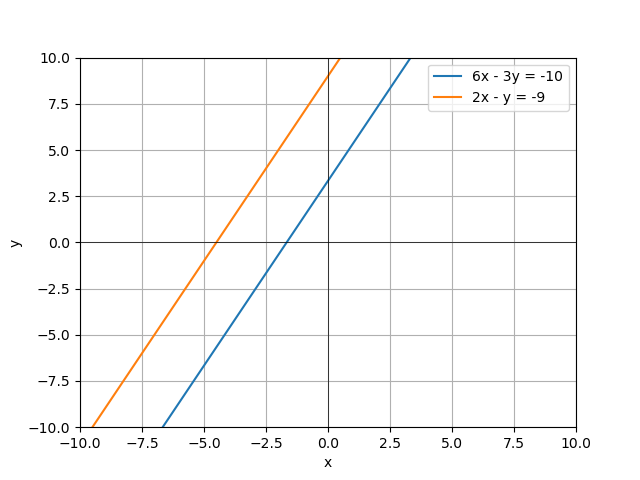
\includegraphics[width=\columnwidth]{figs/fig.png}
	\caption{Plot of the lin $6x - 3y+10$ and $2x-y+9=0$}
 \end{figure}

\end{document}
|
